\chapter{Related Work}
\label{chap:related_work}

This chapter reviews literature and existing work which is of relevance to this study. It is structured in 7 main sections:

\begin{enumerate}
    \item Review of digital and net art conservation theory
    \item Review of archival standards and systems
    \item Review of blockchain, smart contracts and NFTs
    \item Overview of the architecture of Teia and HEN OBJKTs
    \item Survey of representative artworks
    \item Tentative taxonomy of crypto art
    \item Theoretical framework adopted by this study
\end{enumerate}

\vspace{0.5cm}

The review follows a narrative approach, with the goal of understanding the contextual background in which this work is situated. However it should be noted that there was a delimitation in the selection of materials reviewed, as only those which were made available as open access were included. In addition to academic papers, a number of books were reviewed, in the areas of blockchain art, netart, digital art conservation and information systems. A number of web resources in the area of art conservation were also consulted. 

Due to the novel area of networked crypto art, there is not a lot of existing academic literature published in this specific topic. For this reason, the research for this work relied primarily on the existing work of conservation of the Web, the extensive literature on digital art conservation in general, particularly that which focused on code-based art and netart, and also on a review of actual code-based crypto artworks.

\section{Digital and Net Art Conservation}

Due to the lack of existing literature on the conservation of networked crypto art, a reasonably good starting point is the study of digital art, and where possible, focusing on net art.

Net art is an art movement which started in the early 1990s and gained prominence in the middle of the decade, fuelled by the rise in popularity of the World Wide Web \cite{schreiberNetArtShedding2001}. It uses the Internet as a medium, and is usually highly interactive often invoking the participation of the viewer \cite{kholeifInternet_ArtBirthWeb2023}. Although there is no clear consensus on a definition of net art, this study will adopt the definition proposed by Rhizome on their Net Art Anthology: "art that acts on the network, or is acted on by it" \cite{WhatNetArt2017}.
This emphasis on the interaction between the art and the network was famously captured by MTAA in 1997, see \autoref{fig:simplenetartdiag}.

\begin{figure}[h]
    \centering
    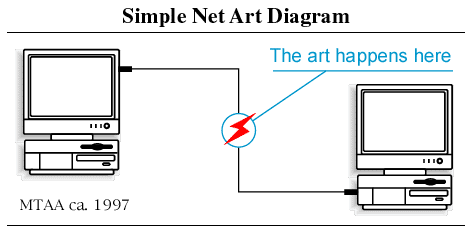
\includegraphics[width=0.75\linewidth]{netartdiagram.png}
    \caption[Simple Net Art Diagram]{Simple Net Art Diagram. Source: MTAA \cite{NETARTANTHOLOGY2016a}}
    \label{fig:simplenetartdiag}
\end{figure}

Net art shares many similarities with networked crypto art. In fact, if we try to set them apart, the main difference between a net net artart artwork and a networked crypto art artwork is that the later is registered on a blockchain, and as per our delimitation of scope, operates exclusively in the digital realm. Thus crypto art can be said to lay at the intersection of net art and crypto art. This allows us to draw the first part of our conceptual framework.


\begin{figure}[h]
    \centering
    \includesvg[width=0.75\textwidth]{netart-crypto-art}
    \caption[Networked crypto art at the intersection of net art and crypto art]{Networked crypto art is at the intersection of net art and crypto art}
    \label{fig:netart-crypto-art}
\end{figure}

Net art belongs to a wider category of digital art, specifically born-digital art, which designates artworks created in a digital format from the outset, and which depends on the technology to operate \cite{innocentiKeepingBitsAlive2013}.

\subsection{What is Conservation?}

As defined in \autoref{sec:definitions} (\nameref{sec:definitions} , page \pageref{sec:definitions}), conservation consists of a number of activities taken toward achieving the long-term preservation of cultural heritage. There is a wide range of such activities, but after a systematic review of digital art conservation literature, the following emerged as the most common:

\begin{itemize}
    \item Aquisition
    \item Archival Storage
    \item Access
    \item Emulation
    \item Migration
    \item Restoration
    \item Reconstruction
    \item Reinterpretation
    \item Documentation
\end{itemize}

The following sections will examine these activities in more detail.

\subsection{Acquisition}

Acquisition is the process that a cultural heritage institution takes to obtain an artifact for conservation. It is normally divided into 3 phases \cite{ahtilaAcquiringMediaArt1998}:

\begin{enumerate}
    \item \textbf{Pre-aquisition}: a pre-assessment of the artifact, to find its condition and whether it can be exhibited sustainably. This assessment includes an estimation of the overall costs, which include acquisition, exhibition, and continuing costs. If the assessment is positive, then the terms for the negotiation of the acquisition contract are drafted.
    \item  \textbf{Acquisition}: the process of acquisition involves negotiation with the vendor or donor, verification that all agreed components were delivered, including preservation materials, and exchange contracts;
    \item  \textbf{Post-acquisition}: work is catalogued and documented, and a long term conservation plan is made, potentially informed by follow-up interviews with the artist.
\end{enumerate}

In a digital context, acquisition is also commonly called \emph{injest}, see \autoref{sub:oais}.

\subsection{Archival Storage}

Cultural heritage institutions involved in conservation of digital art need to develop a robust archival storage strategy. Depending on the size of the institution they may choose to invest in on-site storage, normally in server rooms designed for that purpose, or outsource it to specialised storage or cloud vendors, and in many cases for the purposes of redundancy, both.

In this area the National Digital Stewardship Alliance (NDSA) published authoritative guidelines for industry best practices, see \autoref{tab:ndsa-levels-of-digital-preservation}

These guidelines include the practice of \emph{file fixity}, which consists of the use of checksums or file hashing, as discussed in \autoref{sub:blockchain}, to ensure a file is ``fixed'' or unchanged. It also encourages a well known practice in the archival community known as \emph{Lots of Copies Keep Stuff Safe} (LOCKSS).

Institutions are also adopting storage information systems which comply with the \gls{oais} standard. This standard is of special interest to this work, so it will be examined in more detail in \autoref{sub:oais}.

\begin{table}[h!]
\centering
\captionsetup{type=table} % This makes the caption be treated as a table caption
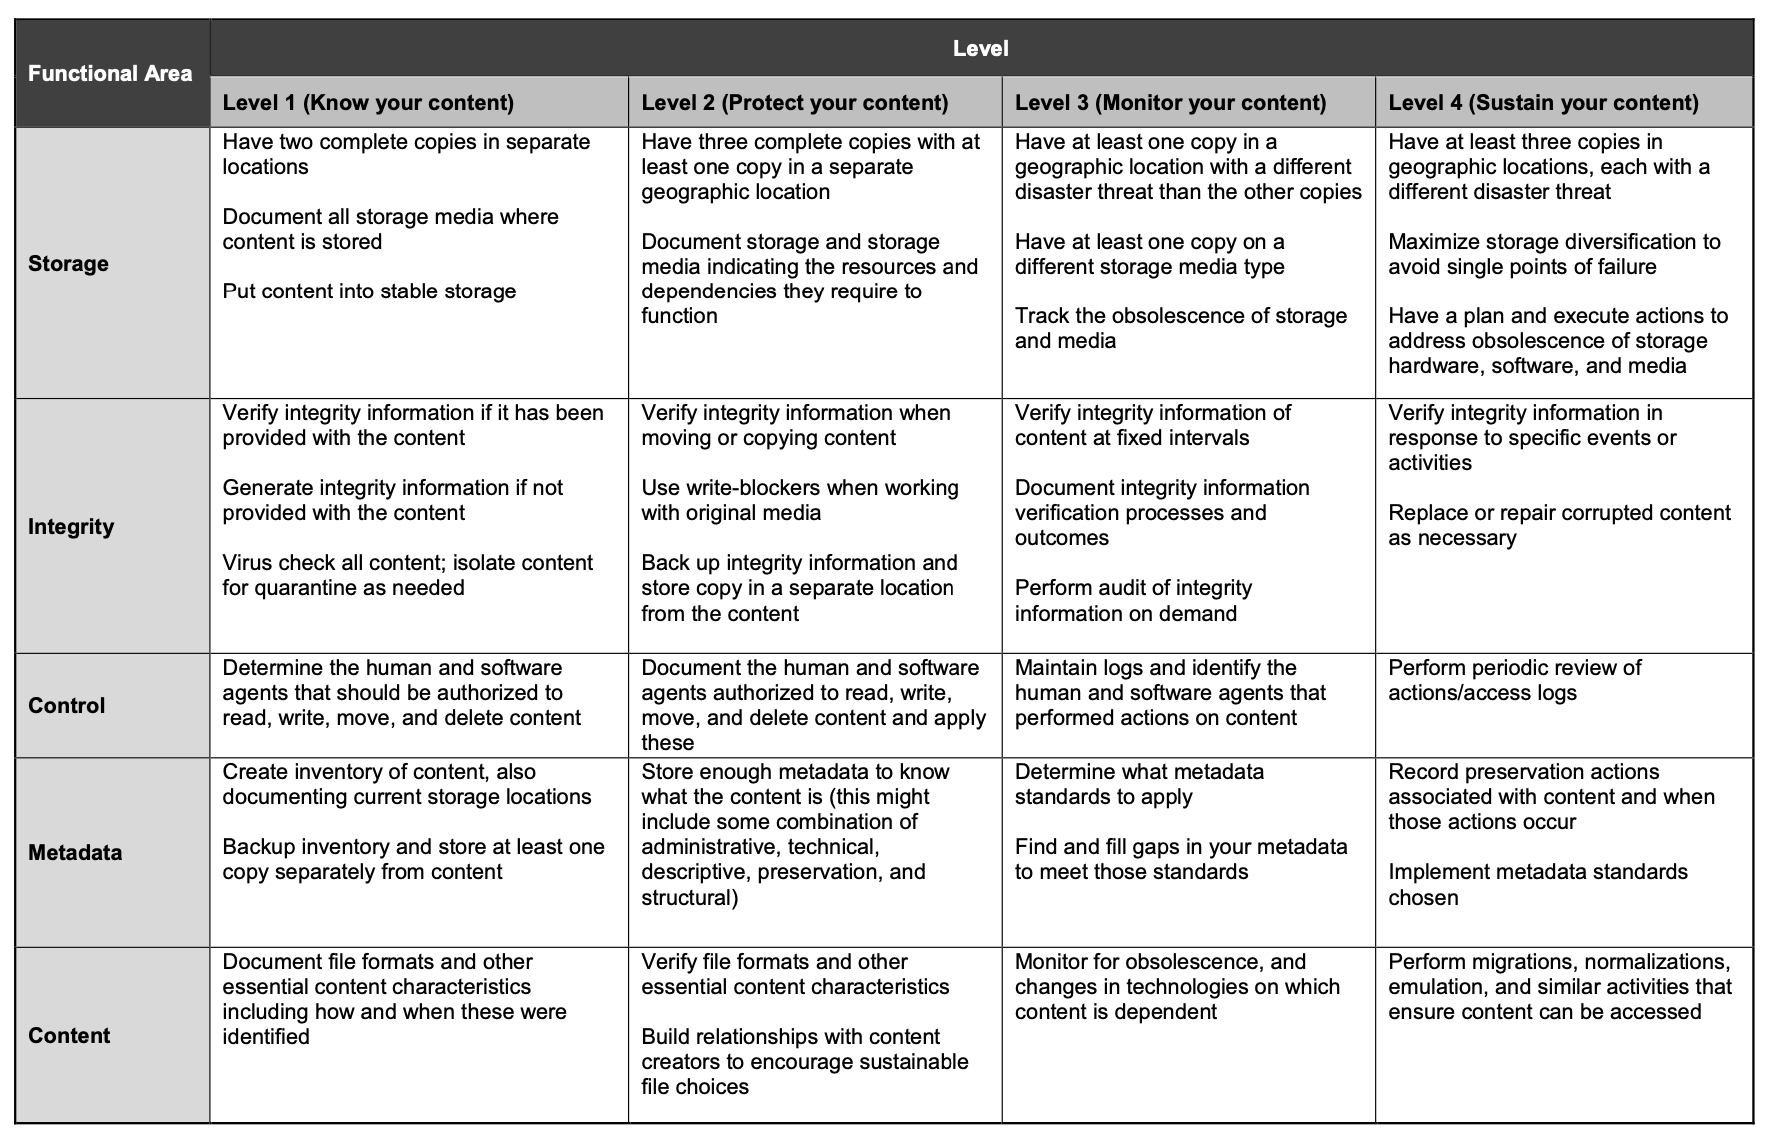
\includegraphics[width=\textwidth]{table-ndsa-matrix.png} % Adjust the width as needed
\caption[NDSA Levels of Digital Preservation Matrix V2.0]{NDSA Levels of Digital Preservation Matrix V2.0. Source: https://osf.io/qd54c}
\label{tab:ndsa-levels-of-digital-preservation}
\end{table}


\subsection{Access}

The archive should provide a user interface, allowing users to browse and search its contents, and in applicable to request copies of materials. In some cases some degree of access control may need to be put in place, in which case the system should provide such a feature. \cite{nationallibraryofaustraliaGuidelinesPreservationDigital2003}

\subsection{Emulation}

Emulation is the recreation of a particular system, either hardware or software, as software which runs in a virtualised environment within another system \cite{rothenbergUsingEmulationPreserve2000}. It is one of the most common methods of preserving digital systems which became obsolete over time.

It is widely used in a variety of contexts, from reviving old video games, such as arcade\footnotemark[1], ZX Spectrum\footnotemark[2], and many other obsolete systems\footnotemark[3], as well as more recent web publishing proprietary systems like Adobe Flash\footnotemark[4] and even obsolete calculators \cite{scottjasonCalculatedMoveCalculators2023}.

\footnotetext[1]{\url{https://www.mamedev.org/}}
\footnotetext[2]{\url{https://archive.org/details/softwarelibrary_zx_spectrum}}
\footnotetext[3]{\url{https://archive.org/details/software}}
\footnotetext[4]{\url{https://ruffle.rs/}}

OldWeb.Today, which combines web-based \gls{emulation} of obsolete browsers, like NCSA Mosaic and Netscape Navigator, with Archive.org's Wayback Machine web snapshots, enables users to experience navigating the web as it was all the way back into the 1990s, see \autoref{fig:oldweb}.

\begin{figure}[h]
    \centering
    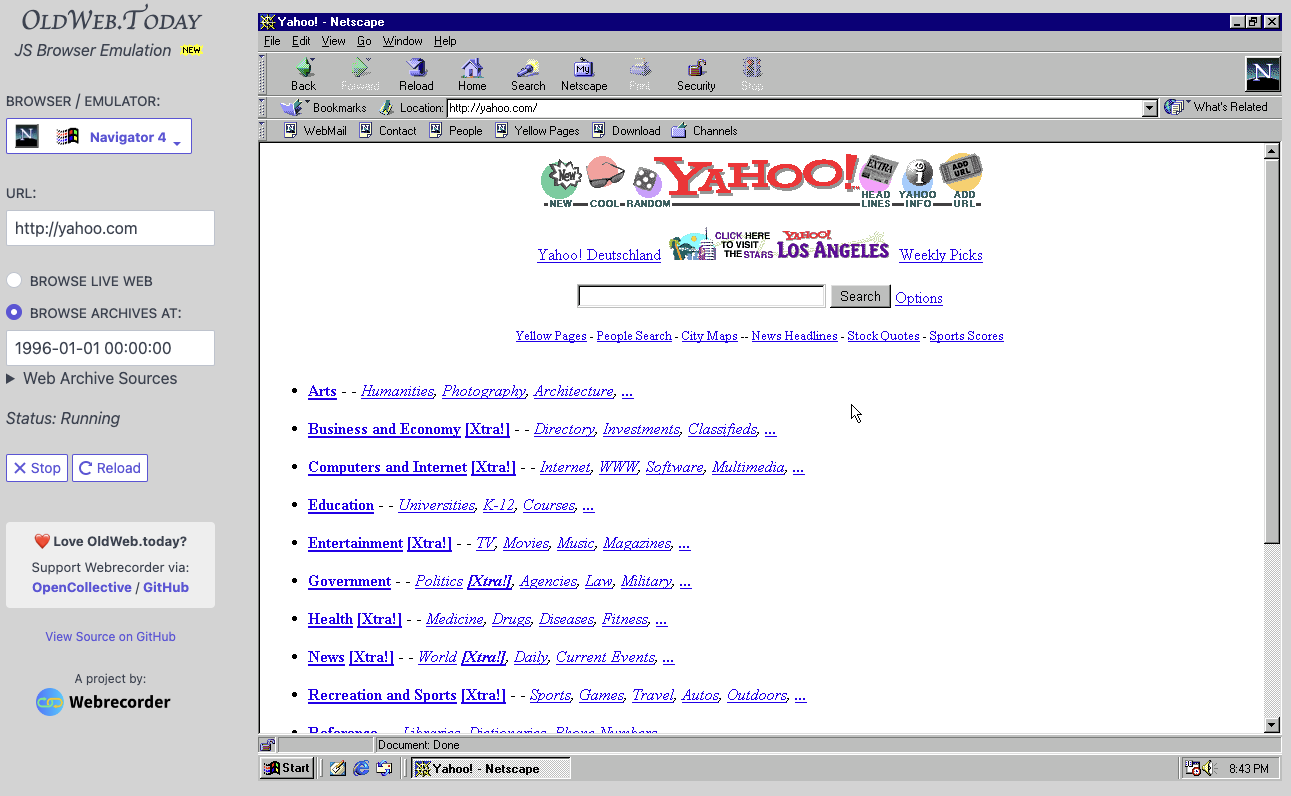
\includegraphics[width=\linewidth]{oldweb.png}
    \caption[OldWeb.Today Browser Emulator]{OldWeb.Today Browser Emulator. Source: https://oldweb.today/ }
    \label{fig:oldweb}
\end{figure}

One challenge of emulators is that, as any other software system, they may have to be readapted to run on more modern hardware. This means that the work of creating and updating emulator software is likely to be an ongoing effort for the foreseeable future.

\subsection{Migration}

Migration of a digital artwork involves moving it from its original technological environment, to a more modern one. However it is often the case that this will result in some degradation of the artwork, due to incompatibilities between the two environments. \cite{huberNewMediaOld2013}

As an empirical example of this, we can use the ACID test v2, which was test web page setup in 2005 by the Web Standards Project to test web browser compatibility with the standards for displaying HTML markup, PNG images, CSS 2.1styling, and data URIs \cite{Acid22024}.

If we access the test page\footnotemark[5] with a modern browser, such as Google Chrome Version 127 on a Mac OS 13.6 operating system, and compare it with the reference image\footnotemark[6], we can see clearly that backwards compatibility with web standards that were in place less than 20 years ago is already decaying.

\footnotetext[5]{\url{http://acid2.acidtests.org/\#top}}
\footnotetext[6]{\url{http://acid2.acidtests.org/reference.html}}


\begin{figure}[H]
  \centering
  \begin{subfigure}[b]{0.45\textwidth}
    \centering
    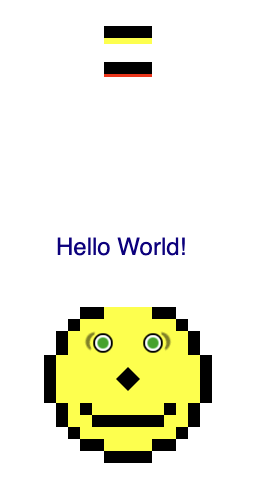
\includegraphics[width=0.50\textwidth]{acid2-test.png}
    \caption{ACID test v2 in 2024}
    \label{fig:image1}
  \end{subfigure}
  \hfill
  \begin{subfigure}[b]{0.45\textwidth}
    \centering
    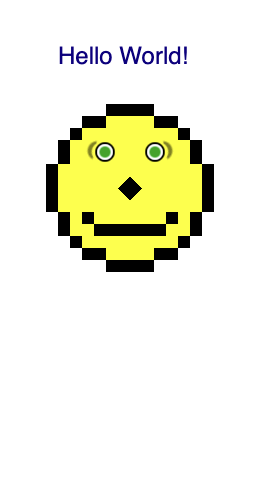
\includegraphics[width=0.50\textwidth]{acid2-reference.png}
    \caption{ACID test v2 reference image}
    \label{fig:image2}
  \end{subfigure}
  \caption{ACID v2 test with modern browser}
  \label{fig:acid2-test}
\end{figure}

This is a reminder that following web standards today is no guarantee of the fidelity of renderings in the future. 

\subsection{Restoration}

Restoration is an umbrella term used for a set of conservation practices "undertaken to restore an object to known preceding states" \cite{dekkerCollectingConservingNet2018}. In general these are meant to be as non-invasive as possible in order to maintain the artworks' authenticity. 

\subsection{Reconstruction}

Reconstruction goes a step further than restoration, as it involves rebuilding parts of an artwork, usually based on extensive documentation provided by the artist, so as to maintain their original intent, although it can be argued that any reconstruction is always susceptible to some degree or reinterpretation \cite{huberNewMediaOld2013}.


\subsection{Reinterpretation}

Reinterpretation represents the most radical intervention in the integrity of an artwork, as it may need to be adapted to a new environment, with new parameters. It may sometimes present itself as the last resort to preserve the artwork and, just like reconstruction, ideally it should be done in consultation with the artists as to maintain its original intention \cite{serexheDigitalArtConservation2013}.


\subsection{Documentation}

Documentation is arguably the most important conservation practice in digital art preservation, being mentioned in the vast majority of articles and books.

Depocas noted that ``sometimes this documentation is the only evidence left of an artwork's existence'' \citeyear[p.145]{depocasDocumentingConservingTechnological2013}.

Several efforts have been initiated by digital art conservation community in an effort to standardise documentation practices.

\subsubsection{Variable Media Network}

The Variable Media Network is a project that provides a set of guidelines and taxonomies, and a questionnaire which can help guide conservators in documenting digital artworks \cite{depocasPermanenceChangeVariable2003}. For example, artworks can be classified as: contained, installed, performed, interactive, reproduced, interchangeable, encoded (our definition of code-based), and networked. Their questionnaire allows the recording of elements such as: stakeholders (persons, institutions, studios), artworks (title, year, description), components (material, environment, interaction), package (contained, installed, performed, interactive), questions (about storage, emulation, migration, reinterpretation), and allows the linking of these elements. For example a stakeholder, like an artist, can be linked to several artworks \cite{VariableMediaNetwork}.

The project also implemented a questionnaire\footnotemark[10] as an interactive web-based application, as illustrated in \autoref{fig:vmnq}.

\footnotetext[10]{https://variablemediaquestionnaire.net/}

\begin{figure}[h]
    \centering
    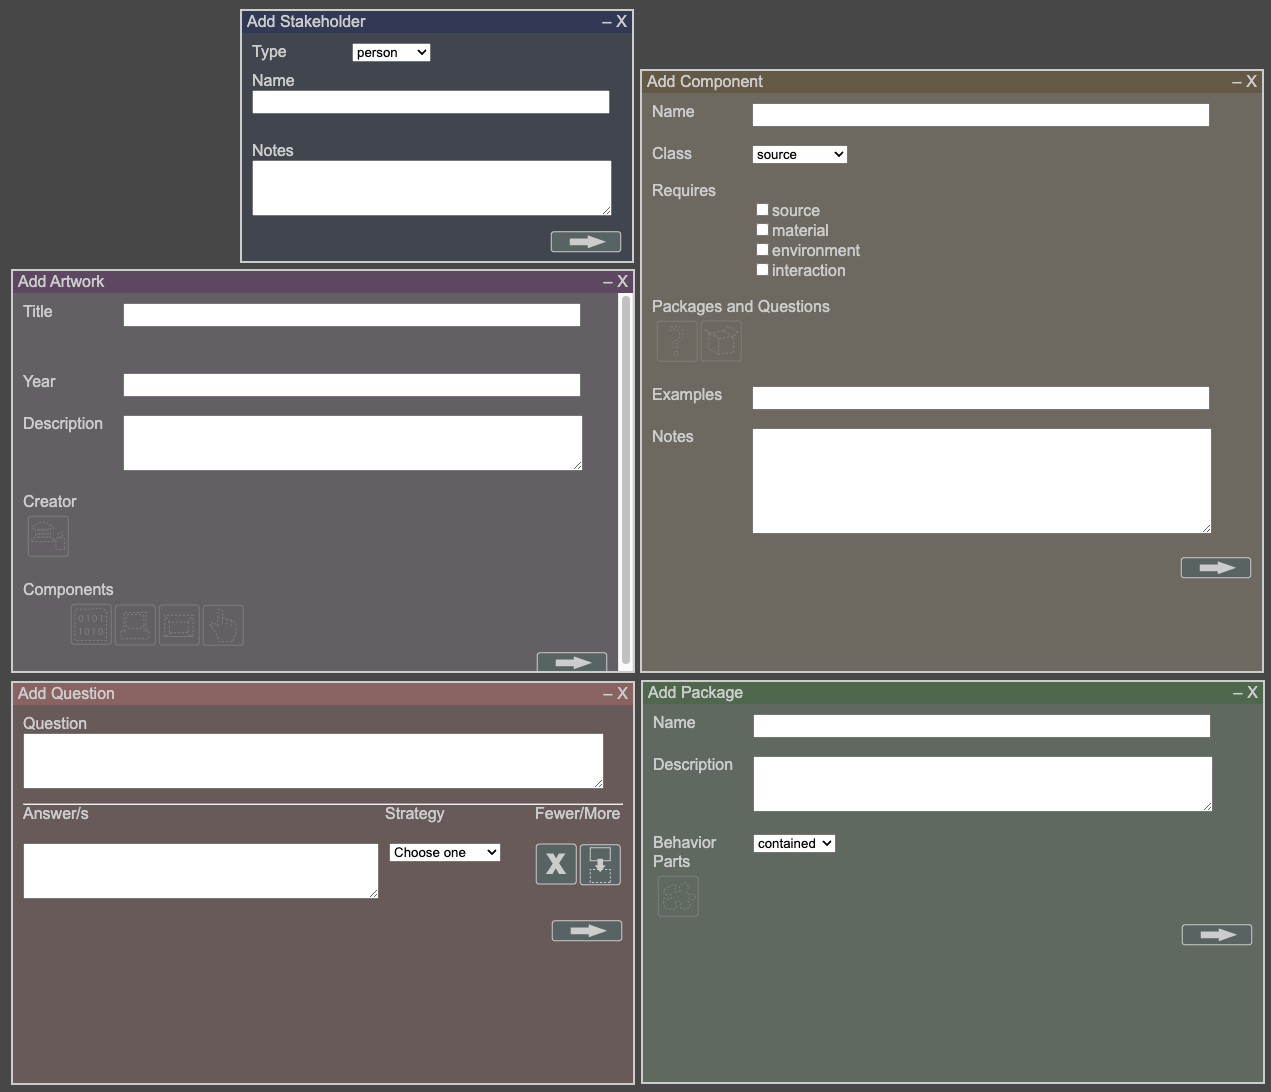
\includegraphics[width=\linewidth]{variablemedianet-questionnaire.png}
    \captionsetup{justification=centering}
    \caption[Variable Media Network Questionnaire]{Variable Media Network Questionnaire. \\ Source: https://variablemediaquestionnaire.net/}
    \label{fig:vmnq}
\end{figure}

\subsubsection{DOCAM Documentation Model}

The Research Alliance Documentation and Conservation of Media Arts Heritage \cite{DOCAM} produced cataloguing and conservation guides, as well as a set of documentation models for the conservation of media art. This model ``offers a structural framework within which all the information pertaining to a work can be assembled, organized, and made accessible'' \cite[p.151]{depocasDocumentingConservingTechnological2013}.

Their model structures the documentation across 4 main lifecycles of the artwork: creation, dissemination, research and custody. See \autoref{fig:docam-model}.

\begin{itemize}
    \item \textbf{Creation}: definition of the concept, presentation method, and required elements its presentation;
    \item \textbf{Dissemination}: presentation and publicity strategies, including installation, presentation, deinstallation and criticism;
    \item \textbf{Research}: activities surrounding the study or critical analysis of a work;
    \item \textbf{Custody}:  various facets of custodial responsibility, such as storage, cataloguing, conservation and preservation;
\end{itemize}


\begin{figure}[h]
    \centering
    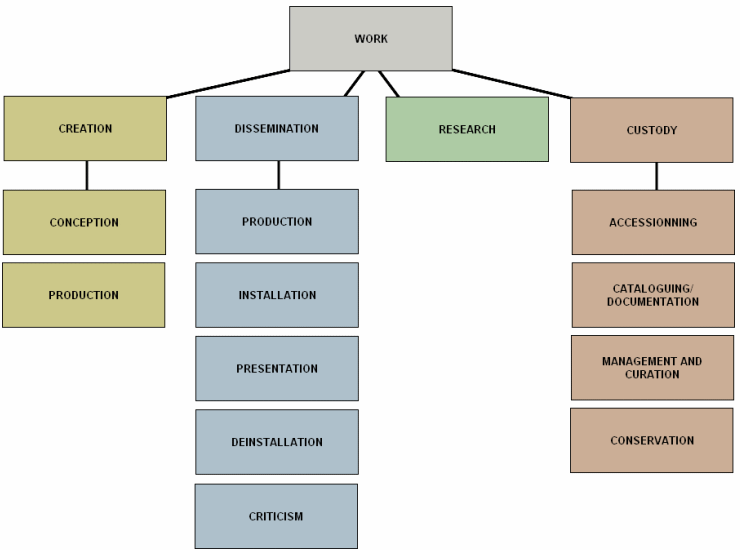
\includegraphics[width=\linewidth]{docam-struct.png}
    \captionsetup{justification=centering}
    \caption[DOCAM Documentation Model - Lifecycle Events]{Lifecycle events of a work as per the DOCAM Documentation Model. \\ Source: https://www.docam.ca/en/documentation-model.html}
    \label{fig:docam-model}
\end{figure}


\section{Archival Standards and Systems}

Digital preservation is not a problem specific to digital art, and several efforts have been made to create standards for the long-term archival of digital assets. The following sections discuss some of the most significant ones.

\subsection{Open Archival Information System (OAIS)}
\label{sub:oais}

The Open Archival Information System (\gls{oais}), an ISO standard, is the standard reference model for the long term archiving of digital data, and is one of the most quoted archival standards in digital art preservation. Its model describes best practices across all stages of a digital asset's life cycle: ingest, archival storage, data management, and access \cite{ccsdsReferenceModelOpen2012}. These stages were taken into account when developing the artifact for this project.

The model makes reference to 3 types of information packages:

\begin{itemize}
    \item \textbf{Submission Information Package (SIP)}: which is the information sent from the producer to the archive 
    \item \textbf{Archival Information Package (AIP)}: which is the information stored by the archive
    \item \textbf{Dissemination Information Package (DIP)}: which is the information sent to a user when requested
\end{itemize}

It also makes recommendations with regards to the metadata that should be attached to each digital asset:

\begin{itemize}
    \item reference (identification) information
    \item provenance (including preservation history)
    \item context
    \item fixity (file checksums)
    \item representation (formatting, file structure)
\end{itemize}


\begin{figure}[h]
    \centering
    \captionsetup{justification=centering}
    \includesvg[width=\textwidth]{OAIS-high-level-data-flow}
    \caption[OAIS High Level Data Flow]{OAIS High Level Data Flow. \\ Adapted from: https://public.ccsds.org/Pubs/650x0m2.pdf}
    \label{fig:oais-high-level-data}
\end{figure}

This model constitutes the gold standard for digital archives, and is quite applicable to an archive of crypto art such as the one developed by this project. As mentioned above, at a very basic level \texttt{ARKIVO} already implements the high level data flows illustrated in \autoref{fig:oais-high-level-data}. However a great deal of work is still required to address aspects of the standard such as migration, interoperability and others.

\subsection{Archivematica}

Archivematica\footnotemark[10] is a web-based digital archive that follows the OAIS standard and integrates with many other data repository systems. It is open source, well designed and reasonably well maintained. However it was not suitable as a base software stack for this project because it relies heavily on web2 style authentication (username and password) and therefore it does not suit the web3 culture that our artifact needs to cater for.

\footnotetext[10]{https://www.archivematica.org/en/}

\subsection{Rhizome ArtBase}

The Rhizome ArtBase is an online archive of digital artworks. At the time of writing it hosts 2318 artworks, ranging from websites, moving images, net art, code-based artworks, and games.

Following are screenshots of the main landing page, and an artwork page.


\begin{figure}[H]
  \centering
  \captionsetup{justification=centering}
  \begin{subfigure}[b]{0.45\textwidth}
    \centering
    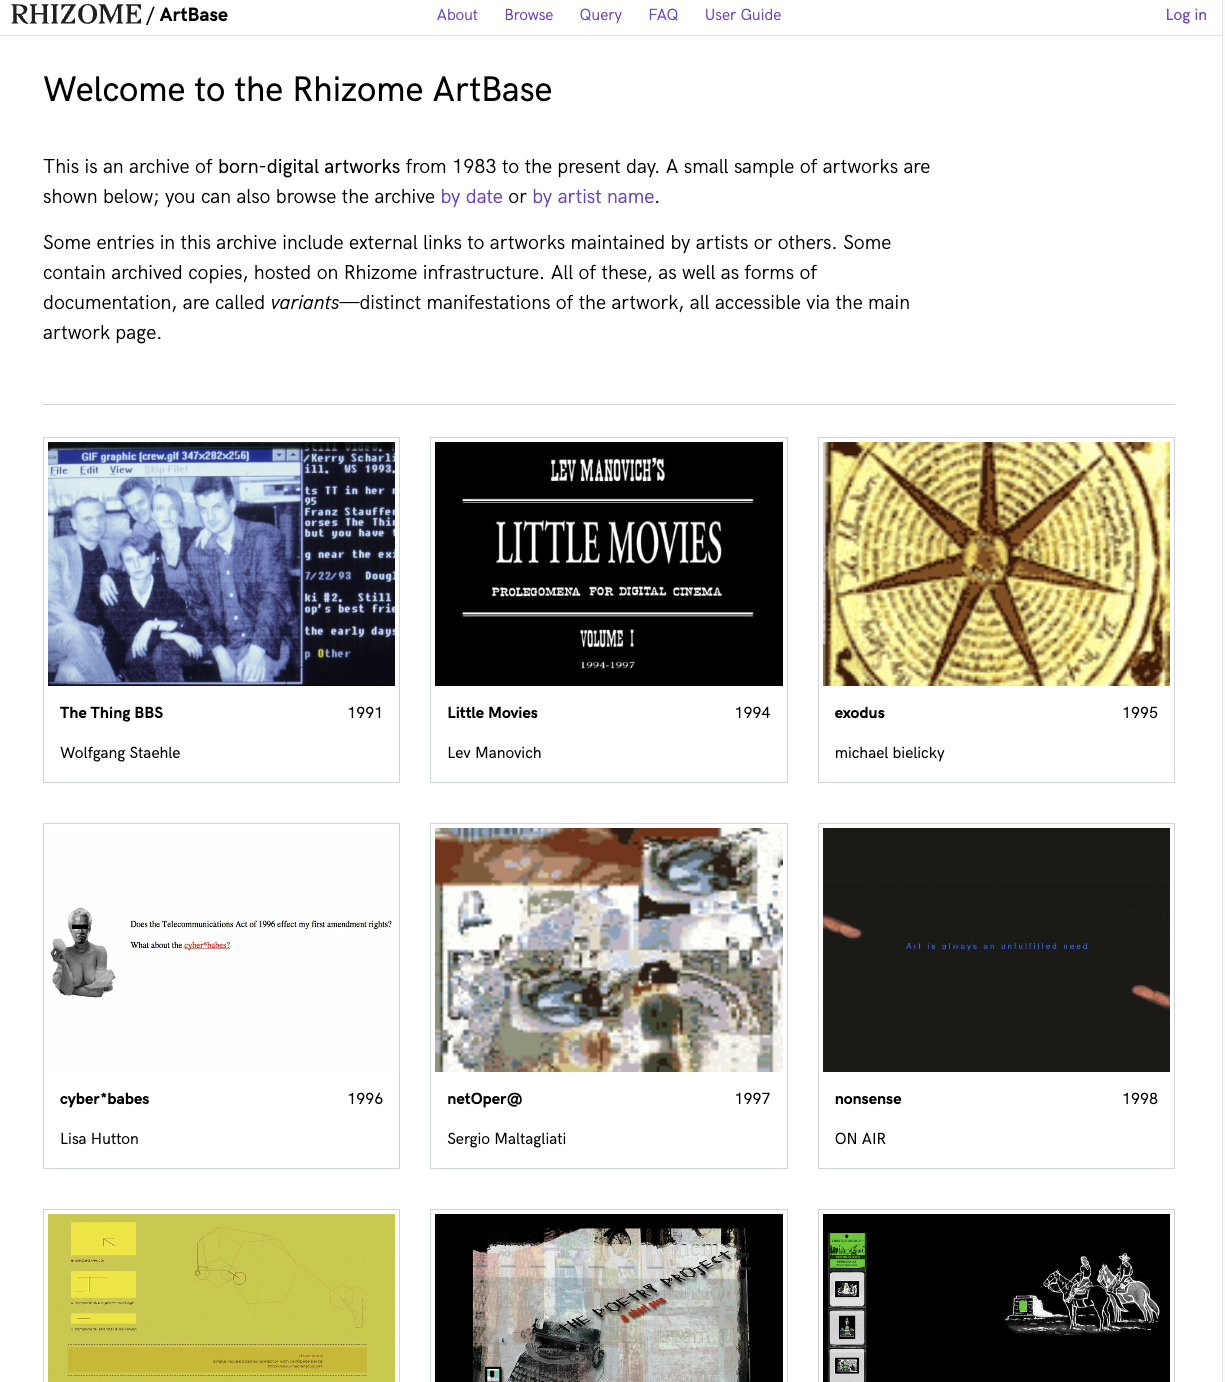
\includegraphics[width=\textwidth]{rhizome-artbase.png}
    \caption{Rhizome ArtBase}
    \label{fig:image1}
  \end{subfigure}
  \hfill
  \begin{subfigure}[b]{0.45\textwidth}
    \centering
    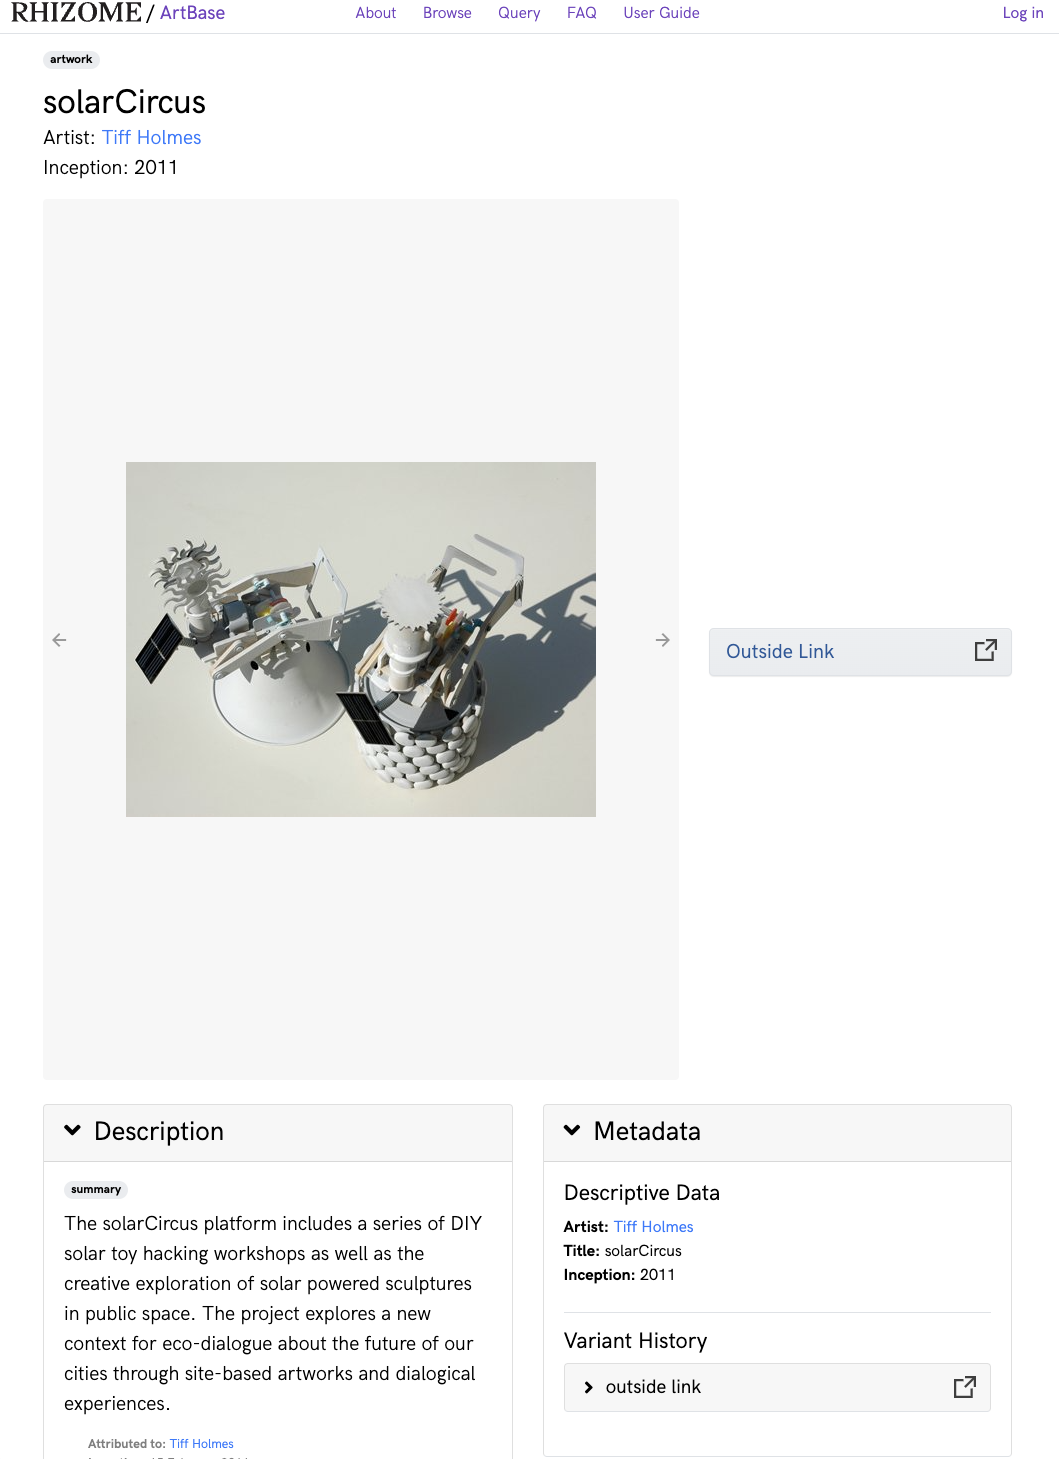
\includegraphics[width=\textwidth]{rhizome-artwork.png}
    \caption{solarCircus by Tiff Holmes}
    \label{fig:image2}
  \end{subfigure}
  \caption{Screenshots of Rhizome ArtBase. \\ Source: https://artbase.rhizome.org/}
  \label{fig:rhizome-screens}
\end{figure}

Each artwork page contains a basic description, and additional metadata about the artwork. It also contains linked objects (normally to the artist's own website), archival copies, or both.

It does not provide a traditional search function, but rather a more powerful query service based on the SPARQL query language, which in theory should allow for complex queries of its Linked Open Data (LOD) infrastructure. However at the time of writing this feature fails run, even the demo queries provided by the system.

Its minimalistic design, which places the artwork first, was a major inspiration for the artifact developed in this work. 

\subsection{Archive.org and Wayback Machine}

Although not specific to art, archive.org undoubtedly constitutes one of the most important archives of web history. It currently hosts 212 PetaBytes worth of web page snapshots, digitised books, videos, audio, images and software \cite{InternetArchivePetabox}.

Unfortunately, due to Teia's client-side and highly dynamic UI, Wayback Machine fails to capture any artworks rendered on Teia's main pages. According to the LOCKSS principle, this is unfortunate, as having another archival copy of the artworks would be advantageous. Although it's possible to manually request snapshots of the IPFS asset itself, bypassing Teia's UI, in practice it would make finding such an artwork very difficult, as most users would be looking for the snapshots of the Teia URLs.

\subsection{WebRecorder and WARC files}

The WebRecorder project develops a number of tools for the recording (archival), and replaying, of webpages, similarly to the snapshots taken by Wayback Machine. These tools range from browser extensions, to desktop applications, and even command line tools and software libraries.

Importantly, snapshots taken by the WebRecorder family of tools conform to the Web ARChive (WARC) file format, which has become a standard in the industry \cite{WARCFileFormat2024}.

Such a feature would be highly valuable for our artifact, however through experimentation it was found that, unlike their desktop tools, the software libraries currently lack the ability to fully capture a web page with all its assets. Instead they only capture a single HTTP request. Lacking this basic single-page crawling ability meant that integration of WARC snapshots will be postponed for future work.


\section{Blockchain Technology, Smart Contracts and NFTs}


\subsection{Blockchain}
\label{sub:blockchain}

The concept behind a blockchain is not new. It was first introduced by Stuart Haber and Scott Stornetta in 1991 in the Journal of Cryptology \cite{haberHowTimeStampDigital1991}. The problem they were trying to solve was: how can we trust historical records when digital media is so easy to manipulate, and how can we do so without having to trust a central authority? Their solution relied on one-way hashing functions.


\begin{figure}[h]
    \centering
    \includesvg[width=0.5\textwidth]{hashing}
    \caption[One-way hashing examples]{Examples of one-way hashing (here SHA1 was used). The same input always produces the same hash. Different inputs produce different hashes, even if the difference is just one character, or even one bit.}
    \label{fig:hashing}
\end{figure}

Haber and Stornetta's solution involved combining the hash of a document into the data input for the next document hash, resulting in a recursive chain of hashes which had an important property: any change to any of the documents, no matter how small, would break the chain of hashes from that point onwards.
By weekly publishing the latest hash of the chain, which they did in the``Notices'' classified advertisements section of a the New York Times \cite{whitakerArtBlockchainPrimer2019}, they effectively created the first time-stamped proofs of the immutability of those digital documents, and arguably the world's first blockchain.

\begin{figure}[h]
    \centering
    \includesvg[width=0.5\textwidth]{hash-chains}
    \caption[Illustration of a chain of hashes]{Illustration of a chain of hashes}
    \label{fig:hashing}
\end{figure}


\subsection{Bitcoin}

Satoshi Nakamoto \cite{nakamotoBitcoinPeertopeerElectronic2008a}  adopted this concept of an immutable data chain and added the required components to turn it into a global decentralised ledger, where financial transactions can be recorded. These components were:

\begin{enumerate}
    \item a peer-to-peer network of nodes running the same software, which validate all transactions added to the ledger 
    \item cryptographic signatures, so that transactions spending or transferring a particular asset are only accepted by the network when signed by the asset's owner
    \item the ordering of transactions into blocks, which are linked together by their hashes
    \item a lottery system that determines which node on the network is eligible to publish the next block
    \item a proof-of-work system with self-adjusting difficulty so that on average only one node is able to win the lottery every 10 minutes. Also the proof-of-work required for altering old blocks becomes exponentially larger with each block added, as an attacker would need to produce more proof-of-work than the rest of the honest nodes combined
    \item a fungible token, bitcoin, which is used to economically reward nodes who successfully publish blocks and is the native asset traded on the ledger
    \item in addition to block rewards, block producing nodes (miners) also receive fees paid by each transaction which was included in their block
\end{enumerate}

\vspace{0.5cm}

Although the blockchain contains a full history of all transactions ever made since its inception, Bitcoin stores the current state of the ledger, in other words, the index of who owns what, in a set of unspent transaction outputs (\indexacronym{utxo}). As the name suggests, this is the list of all transactions which have not yet been spent by their recipients.

With his invention, Bitcoin, Satoshi created the first decentralised cryptocurrency, which exhibits several key properties:

\begin{enumerate}
    \item \textbf{Decentralisation}: peer-to-peer network of nodes, operates without any central authority
    \item  \textbf{Censorship resistance}: transactions cannot be stopped of censored by any central authority
    \item  \textbf{Permissionless}: anyone with access to the Internet can download the software and participate on the network
    \item  \textbf{Immutability}: transactions added to the blockchain become immutable, as explained above
    \item  \textbf{Transparency}: all transactions on the ledger are public, and independently verifiable, removing the need for trust (trustless)
\end{enumerate}

\vspace{0.5cm}


\subsection{Ethereum}

As mentioned in the Introduction, Ethereum built on the concept of a blockchain, but unlike Bitcoin it does not use a UTXO approach. Instead, it uses an account-based model as a representation the state of the ledger. There are two types of accounts in Ethereum: Externally Owned Accounts (EOAs) which are controlled by a person's private key and are used to send and receive assets; and Contract Accounts which contain code that gets executed when it receives a transaction from an EOA. The code is executed by the Ethereum Virtual Machine (EVM) which makes changes to the persistent state storage, see \autoref{fig:smartcontract}.

\begin{figure}[h]
    \centering
    \includesvg[width=0.75\textwidth]{smartcontract}
    \caption[Diagram of Smart Contract]{Diagram of Smart Contract}
    \label{fig:smartcontract}
\end{figure}

Just like in Bitcoin, transactions in Ethereum must pay a fee to the block producers, called gas fee. In the case of interactions with smart contracts, the gas is consumed during the execution of the code, with each instruction (opcode) costing a varying amount of gas corresponding to the computational complexity of that instruction. Any unused gas is returned back to the EOA. Gas is paid in Gwei, which is a denomination of Ether, Ethereum's native cryptocurrency.

Ethereum standards, like ERC-20, allow the creation of fungible tokens which can be traded across different wallets and \gls{decentralised application}s (\indexacronym{dapp}s) built on Ethereum \needcite, which led to the \gls{initial coin offering} (\indexacronym{ico}) hype of 2017. \needcite


\subsection{Non-Fungible Tokens}

The ERC-721 standard is used for the creation of unique and non-divisible NFTs, each with a unique identifier, such that they are not fungible as their ERC-20 counterparts.
Due to the limited storage available on the blockchain, the ERC-721 standard defined as part of its \texttt{ERC721Metadata} a \texttt{tokenURI} field which should point to an external location where the actual NFT metadata should be stored. In turn, this metadata should follow the ERC721 Metadata JSON Schema, and includes the name and description of the NFT, and another URI, this time to the actual NFT media asset \cite{ERC721NonFungibleToken}.

%\begin{lstlisting}[style=jsonCode,caption={ERC721 Metadata JSON Schema}] 

\todo provenance

\begin{lstlisting}[language=HTML, caption={ERC721 Metadata JSON Schema}]
{
    "title": "Asset Metadata",
    "type": "object",
    "properties": {
        "name": {
            "type": "string",
            "description": "Identifies the asset to which this NFT represents"
        },
        "description": {
            "type": "string",
            "description": "Describes the asset to which this NFT represents"
        },
        "image": {
            "type": "string",
            "description": "A URI pointing to a resource with mime type image/* representing the asset to which this NFT represents. Consider making any images at a width between 320 and 1080 pixels and aspect ratio between 1.91:1 and 4:5 inclusive."
        }
    }
}
\end{lstlisting}

Even though some early NFT marketplaces stored their NFT metadata and assets in private servers, leading to a loss of the assets when they shutdown \cite{gallenHistoryNFTMarketplaces2023}, nowadays most marketplaces store these in decentralised file storage networks like IPFS and ArWeave, which are more resilient  see \autoref{sec:offchain_storage} - \nameref{sec:offchain_storage}.


\begin{figure}[h]
    \centering
    \includesvg[width=\textwidth]{nft-diagram}
    \caption[Components on an NFT]{Components on an NFT}
    \label{fig:nftcomponents}
\end{figure}


\subsection{Hyperstructures}

\todo https://jacob.energy/hyperstructures.html

\subsection{Off-Chain Storage}
\label{sec:offchain_storage}

As mentioned above, in order to avoid single-points of failure while storing NFT assets off-chain, most NFTs use decentralised file storage solutions to store their assets. Several projects offer such solutions, but lately two projects have gained relevance in this area: \gls{interplanetaryfilesystem} and ArWeave. 


\subsubsection{InterPlanetary File System}
\label{sec:ipfs}

IPFS is a suite of protocols for organising and transferring data over a \gls{peertopeer} network, using content addressing rather than location addressing, such as domain names or IP addresses.
Content addressing works by hashing the contents of the file, or smaller chunks when the file is big enough. This hash is known in IPFS as a \gls{contentidentifier}. IPFS then uses these CIDs to organise the assets in a Merkle \gls{directed acyclic graph} allowing for efficient storage and retrieval.
CIDs are mapped onto the nodes (peerIDs) which host them, using a \gls{distributed hash table}. Through network gossiping the nodes can quickly find a peer which hosts a CID. Nodes also cache CIDs which are retrieved through them, temporarily increasing their availability on the network.
However cached CIDs are eventually garbage collected. To ensure the long term availability of a file on the IPFS network, at least one node must \emph{pin} that content, which is to say, it prevents its own garbage collector from removing it, and advertises itself a host of that CID.
Since a CID is a hash of the content it assures the immutability chain between the on-chain NFT record and its off-chain asset.
For those who do not wish to run their own IPFS nodes in order to pin data, there are commercial services available which will do it for a fee, such as Pinata\footnotemark[7], and Infura\footnotemark[8]. There is also Filecoin\footnotemark[9], a blockchain project which offers a decentralised marketplace linking storage node providers with paying users.

\footnotetext[7]{https://www.pinata.cloud/}
\footnotetext[8]{https://www.infura.io/}
\footnotetext[9]{https://filecoin.io/}


\todo mention ClubNFT

\subsubsection{ArWeave}
\label{sec:arweave}

ArWeave is an alternative to IPFS. It relies on a blockchain architecture to provide permanent storage but, unlike traditional blockchains which suffer from scalability issues in terms of storage, ArWeave nodes shard the data amongst themselves, rather than keeping a full copy of the data in each node.
It also uses a similar content addressing strategy to IPFS and, unlike IPFS, it only requires a one-off payment for perpetual data storage (where perpetual is defined as at least the next 200 years) \needcite

\subsection{On-Chain Storage}

It should be noted that even thought the majority of NFTs follow an off-chain strategy for asset storage, some NFT projects seek to host all their assets directly inside one or more smart contracts, in what is called on-chain storage. The rationale is that on-chain storage is the safest type of storage, since both the NFT and its metadata and media are stored in the same medium. Even though this argument has some merit, it is not without controversy. As more data is added to a blockchain it increases the storage costs for nodes, which can compromise on the level of decentralisation of the network. For this reason many blockchains look for strategies to reduce the storage requirements, for example, by allowing classes of nodes to prune some parts of the data leaving only a much smaller subset of nodes as fully archival nodes. Since multipurpose blockchains are meant to cater to a wide variety of use cases, the argument against on-chain storage of NFT media is that it represents a tragedy of the commons problem \needcite .


\subsection{Provenance}

Atomic Form combines the best of IPFS and Arweave into a single solution \cite{maneliusExtendingNFTMetadata2024}


\subsection{Copyright Implications}
\label{subsec:chap2_copyright}

There is a general consensus throughout crypto art that the act of collecting an \indexacronym{nft} does not grant the collector any copyrights over the NFT's original artwork, which remain with the artist. However the practice of NFT marketplaces engaging in cross-listings, which means displaying the artwork for sale on platforms other than the one where the artist minted the work originally, is widespread. It's a practice that is not only accepted, but arguably even appreciated by artists, who gain a wider platform for displaying, and potentially selling, their artworks. This is something that would not normally happen with a museum or other traditional institutions, who always have to go through a step of acquisition of the artwork, along with conservation specific contract signing, before displaying or applying conservation techniques to it.

For the design of our artifact, this means that merely displaying an artwork on an art conservation platform, by itself, should not not constitute a problem. However if the platform engages in automatic classification and displays such metadata along with the artwork, it may raise issues, as the artist may not agree with a particular classification or intervention. This is an area which needs further attention in future work.





\subsection{NFT Marketplace Restrictions}

It should be noted that some NFT marketplaces apply restrictions to networked artworks. This can be for a number of reasons.
For example, OBJKT.com applies a security warning by default, with an option to disable it.


\subsection{Main Issues}

\subsubsection{Scalability}

One key aspect to remember is that adding more nodes to a network does not improve network scalability if each node must replicate the exact same computation as every other node, which is the case with most consensus and block validating nodes on a blockchain. Of course such wide replication of computation is still desired, for decentralisation purposes, as discussed in \ref{sec:lit_review:decentralisation}


\subsubsection{Moore's Law and Data Storage}

\subsubsection{Economic Sustainability}

mention VDP, its role in wg3.2 (beneficiaries), and how the idea spread to other marketplaces (https://docs.fxhash.xyz/pricing-and-supply)





\subsubsection{Code Security}

One aspect that current digital and net art conservation theory does not cover, but which is a major concern for code-based crypto art is that of security.

NFT marketplaces have a global reach. Anyone can publish a code-based artwork, which is essentially a web application, and have it accessed by hundreds or even thousands of users. To make matters worse, the majority of these NFT marketplace users are likely running crypto wallets on their devices which could be holding significant sums of cryptocurrency and NFTs. This makes NFT marketplaces a potential honey pot for malicious actors who will looking for the opportunity to drain the assets from users wallet. Attacks can either be direct by minting a malicious NFT, or indirect by infecting an open source library which may be used as a dependency by honest NFT artists. This kind of backdoor attack has already happened in the crypto industry when a malicious actor took over the maintenance of a popular javascript NPM module which was used as a dependency in the crypto wallet CoPay \cite{haworthPopularJavaScriptDependency2018}.

Even though addressing the security aspect of crypto art may seem to fall outside the scope of conservation efforts, the fact is that if a conservation tool is already automatically downloading and running artworks in a sandbox in order to snapshot them and preserve their evolution, then it is logical that it should also serve a useful function in this regard.

The area of malware scanning is well established, and it normally involves comparing the target software agains signatures of well known malware.


Strategies can involve code similarity checks \cite{ragkhitwetsagulComparisonCodeSimilarity2018} and particularly in JavaScript \cite{alfagehCloneDetectionTechniques2020} where an artwork's code can be compared against well known wallet code.


Early detection systems based on machine learning \cite{schuttEarlyDetectionMalicious2012}, detection of malicious obfuscated JavaScript code \cite{likarishObfuscatedMaliciousJavascript2009} \cite{fassJaStFullySyntactic2018}, malicious code detection based on semantic analysis \cite{fangDetectingMaliciousJavaScript2020}.


\todo ESLint


However, research into techniques of camouflaging malicious code in a benign \gls{abstractsyntaxtree}
\cite{fassHideNoSeekCamouflagingMalicious2019} serves as a timely reminder that this security minded endeavour may always become a cat and mouse game.


This can also aid in identifying potential outdated libraries which could contain vulnerabilities or even current libraries which were attacked by hackers, looking to add backdoors or other crypto exploiting code.








\section{The Web3 Culture}


\subsection{Decentralisation}
\label{sec:lit_review:decentralisation}



Crypto attempts to replace hierarchical systems of power, where rules are ultimately enforced by the use of violence, which a non-hierarchical system where ``good'' and ``bad'' behaviours are encouraged or discouraged via economic incentives and/or penalties.



\subsection{Social Contracts, Immutability and Hard Forks}


\todo : explain why I changed my stance on code is law.

This section will focus on one of crypto's core \emph{raisons d'être}, trustlessness.

The term trustlessness, does not mean untrustworthy. Rather it represent's an effort to make trust obsolete, replacing it with transparency and a-priory agreed social contracts. These social contracts, represented by code, both at the blockchain protocol level, as well as written into smart contracts, become immutable agreements, and self-executing rules of engagement. This concept is so deeply engrained into the crypto culture that any scenarios that rely on individual's trustworthiness are only considered when absolutely unavoidable.

Smart contracts play an important role in this concept, because once instantiated in a blockchain they become, by default, immutable. Participants that rely on the smart contract still need to verify that the code does what it is supposed to, and unintended and hard-to-find bugs are not only possible but unfortunately a common occurrence in this early stage of the smart contract industry. Even though these bugs can be exploited, leading to consequences which run counter to the intended social contract, the crypto community accepts this risk and tries to mitigate it with stricter contract development processes, and reviews and verifications. However, a smart contract which is purposefully designed to be mutable (a possibility under some circumstances) or which gives its creator or administrator powers that would require trust by the community on them, are naturally seen with suspicion and even counter to the accepted crypto culture values. In the early days of \indexglossary{ethereum} a name was given to this type of code-based social contract: rule of code.

An important feature of immutable social contracts is that they prevent, or at least minimise, the unilateral ``cheating'' by any participant in a transaction or a serie of transactions. In crypto, the act of cheating other participants is called a ``rug pull'', which means the symbolic act of ``pulling the rug out from under the feet of the victims'' leaving them off-balance and causing them to fall.

Immutability, however, does bring some inconveniences. Some times the immutable code fails to represent the expectation of the social contract, and this can happen for a number of reasons. For example, the code could have an unforeseen consequence due to a bug. Other times the needs of the community change with time and the social consensus evolves in ways which are incompatible with the original code. In some cases this evolution can even cause major fissures in the community, leading to a breakup in consensus, with major splits in the opinion of the best way forward. In these cases the immutable code is unable to adapt to a new reality, and the community has no option but to leave behind the original protocol, and jump to a new, modified protocol. We call this phenomenon a \emph{hard-fork}.

There were notable hard-forks in the history of crypto (mention BTC/BCH, ETH/ETC, etc)

Perhaps most importantly is that every participant in an activity is satisfied that their expectations are met by the system, and where opinions between them evolve and diverge, that the system provides a satisfactory and fair resolution to all stakeholders. 

\subsection{Why Decentralisation?}
(looking for a better heading. why do we need trustllessness, immutabilty, censorship resistence, etc)

Activism through digital art, see \cite[p.~212]{hopeDigitalArtsIntroduction2014} , benefits greatly from low barriers of entry, lack of gatekeepers, and censorship resistance (both as infra resilience, and social structures), but how can it be counter-balanced with curation of content, policing of copy mints or copyright infringement, removal of illegal material (i.e. child porn, etc).

Decentralisation as a way to remove single-points-of-failure, thus resilience to attack, was an intentional design decision of ARPANET, which led to the Internet we know today. \cite[p.10]{paulDigitalArt2015}



\section{A New Type of Art}

This thesis invites readers to look at networked art under a new light of sensorship-resistant long-lived preservation, powered by decentralised technologies. Rather than create its own visual aesthetic, this new kind of art may be characterised by a common set of processes and underlying architectures that afford it with the kind of long-lasting characteristic that is seldom attributed to digital medium art.
Another factor that distinguishes it from previous net art is the ability of art pieces to be ``aware'' of their own existence in the marketplace, allowing them to react to actions such as being put up for sale, being sold, the monetary amounts involved, who owns them, etc.
In theory, a piece of art could be created in such a way as to 'earn' a stipend from each sale, and through its own trading activity eventually earn enough as to be able to 'purchase' itself from its human owners, and gain some sort of freedom, or emancipation.
Futhermore, it attempts to blend the seemingly conflicting forces of preservation and evolution.

\subsection{Art as Revolution}

``If revolution can give art its soul, then art can give revolution its mouthpiece'' - Anatoly Lunacharsky

TODO: Refer to ``Art and Revolutio'' by Gerald Raunig (available in UMAC lib: NX 180 R45 Rau 2007)

Walter Benjamin hailed the liberatory and transformative effects of mechanical reproduction on art, suggesting that ``mechanical reproduction erodes the 'aura' of a work of art, which results from its unique existence in a time and place, which revolutionized the social function of art and allowed it to be used for politics rather than ritual''. (Benjamin, 2002: 103-6 - cited in \cite[p.3]{gereArtTimeTechnology2006}






\todo ---------
This thesis contributes to the body of knowledge in the following ways:

It proposes a new taxonomy for categorizing xxx which takes into account yyy, and zzz.

Using this new taxonomy an extensive review and categorization of xxx was undertaken and is available online at https://abc.xyz

It contributes to the field of digital art preservation by combining xxx with yyy in a novel way, and provides evidence of its efficacy in findings nnn.

It demonstrates de economic viability of running decentralised infrastructure by incentivising xxx via the use of zzz, as seen in chapter yyy.

In the field of information systems, it studies and reports on the application of xxx and yyy in the context of zzzz

In conducting the research, the efficacy of using methodology xxx was tested in the context of uuu, revealing limitations yyy and zzz.
\todo --------


Digital assets like \gls{nonfungibletoken} are transforming the art world. An \indexacronym{nft} is a unique digital asset verified using blockchain technology.
This document discusses various examples (EX) of digital assets and their conservation techniques. This is the nature of the \gls{nonfungibletoken}.



\subsection{Historical Consensus - Conservation of Bugs}

One interesting side-effect of maintain global consensus is that every full node must independently validate the whole chain, from it's genesis block until the latest block, which is commonly called the ``head'' of the blockchain. This means every full node, no matter how recently implemented, must be able to replicate every historical consensus rule, including any bugs in early node software, such that all historical block validation proceeds exactly as it did originally. Failure to replicate such bugs would potentially result in modern nodes considering historical blocks as invalid, hence refusing to follow the main historical chain and therefore forking the chain.




















\section{Teia and HEN OBJKT architecture}

In order to understand the overall structure in which OBJKTs exist, we will examine the architecture of the Teia platform.

\begin{figure}[H]
    \centering
    \includesvg[width=\textwidth]{hen-teia-components}
    \caption[Teia and HEN OBJKT architecture]{Teia and HEN OBJKT architecture}
    \label{fig:teia-arch}
\end{figure}


\todo change section title and complete this, with diagrams

\todo mention how OBJKTs do not show their native rendering resolution


\section{Survey of Code-Based Crypto Art}


\label{sec:survey-crypto-art}


\subsection{Blockchain as the Medium}

Early work by Rhea Myers, predates NFTs.

Mad Dog Jones Replicator (2021) - uses an off-chain server (under control of the artist) as an oracle which sends "paper-jam" events to the artwork's smart contract.



Early bitcoin inscribed ASCII artworks.

McCoy early work on Namecoin (2014)


Rhea Myers "Token Equals Text" (2019)

DEAFBEEF

Entanglement by Bjork (have permission for screenshots)


Tezos as the art chain (mention participation in basel


\todo mention Adam, as it is used as an example in the protyping


\todo

\begin{figure}[h]
    \centering
    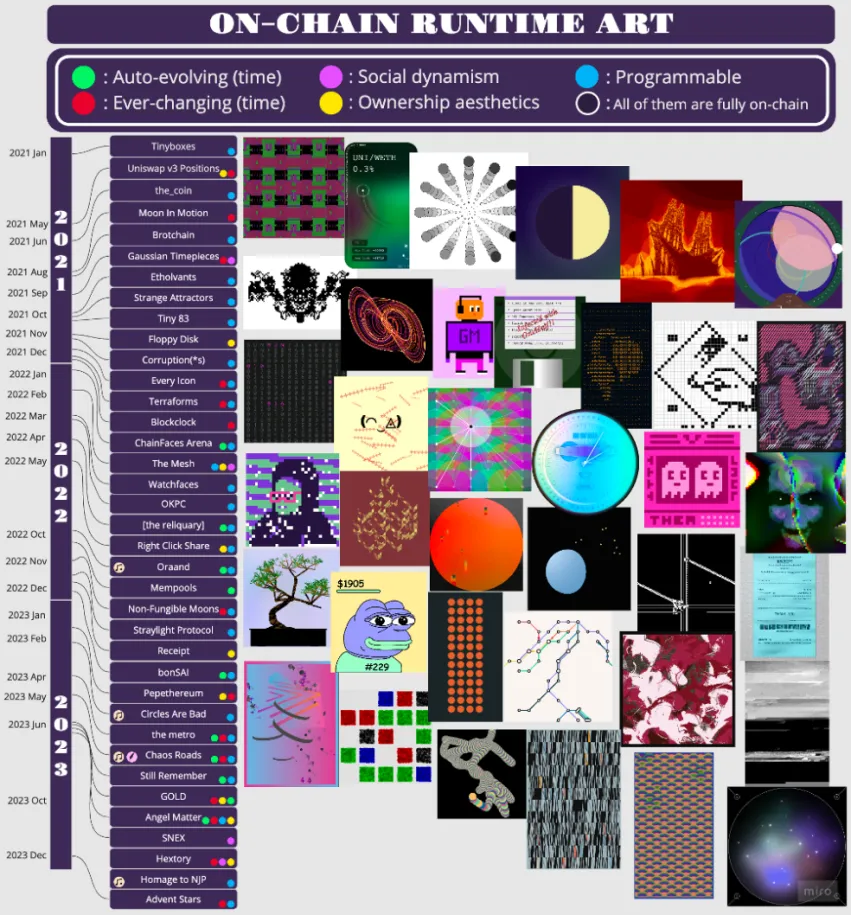
\includegraphics[width=0.75\linewidth]{chainleft-taxonomy.png}
    \caption[Onchain Runtime Art]{Onchain Runtime Art by @chainleft. Source: https://x.com/ChainLeftist/status/1757802497626767455}
    \label{fig:onchainruntimeart}
\end{figure}


Chainleft kindly shared a more detailed description of each category by private message, which can be found in \nameref{appx:chainleft-taxonomy}, page \pageref{appx:chainleft-taxonomy}.









\section{Tentative Taxonomy of Code-Based Crypto Art}
\label{sec:interactivity}

\todo MUST DO THIS, because it's referred to from \autoref{subsec:capture-interactive}.





\todo mention steve jones overlaid menu for dealing with changes in API URLs. these are methods of dealing with the mutable dependency dilemma!


\subsection{Self-Awareness}


\subsection{Viewer Interactivity}

\subsection{Network Interactivity}

\subsection{Time Interactivity}

\subsection{Self-Contained Data Driven}

\subsection{LocalStorage Interactivity}


\subsection{Determinism}

This section deals with whether artworks are deterministic in the way they are rendered or whether there is an element of randomness that even given all the same starting conditions, the artwork will look very different each time. This categorisation is important for conservation because a nondeterministic artwork will be dificult to monitor from a browser obsolescence point of view, especially when using image difference between consecutive snapshots of the artwork. In the case of a non-deterministic artwork, the snapshots will be so different that they become ineffective in detecting changes due to browser version upgrades or other changes in web specifications overtime. In this context, the challenge is to differentiate between a deterministic animated artwork, and a nondeterministic artwork. This challenge exists, because even if an artwork is deterministic, unless there is a way to snapshot the exact same frame across all the snapshots then any image difference comparisons will result in exaggerated differences. In this case we may need to employ more advanced animation frame comparison algorithms, such that the sequence of the animation can be compared across snapshots, and these may involve the recording of the animation, rather than just taking a single snapshot in time. Of course, such a strategy has trade-offs, and in this particular case the trade-off would be a much larger snapshot file size, which will then impact on the overall economic sustainability of the archive.

It should be noted that, determinism is also a reason why fxhash moderates any networked NFT minted on their platform. See \autoref{fig:aliak-data-as-landscape} for an example.

\begin{figure}[h]
    \centering
    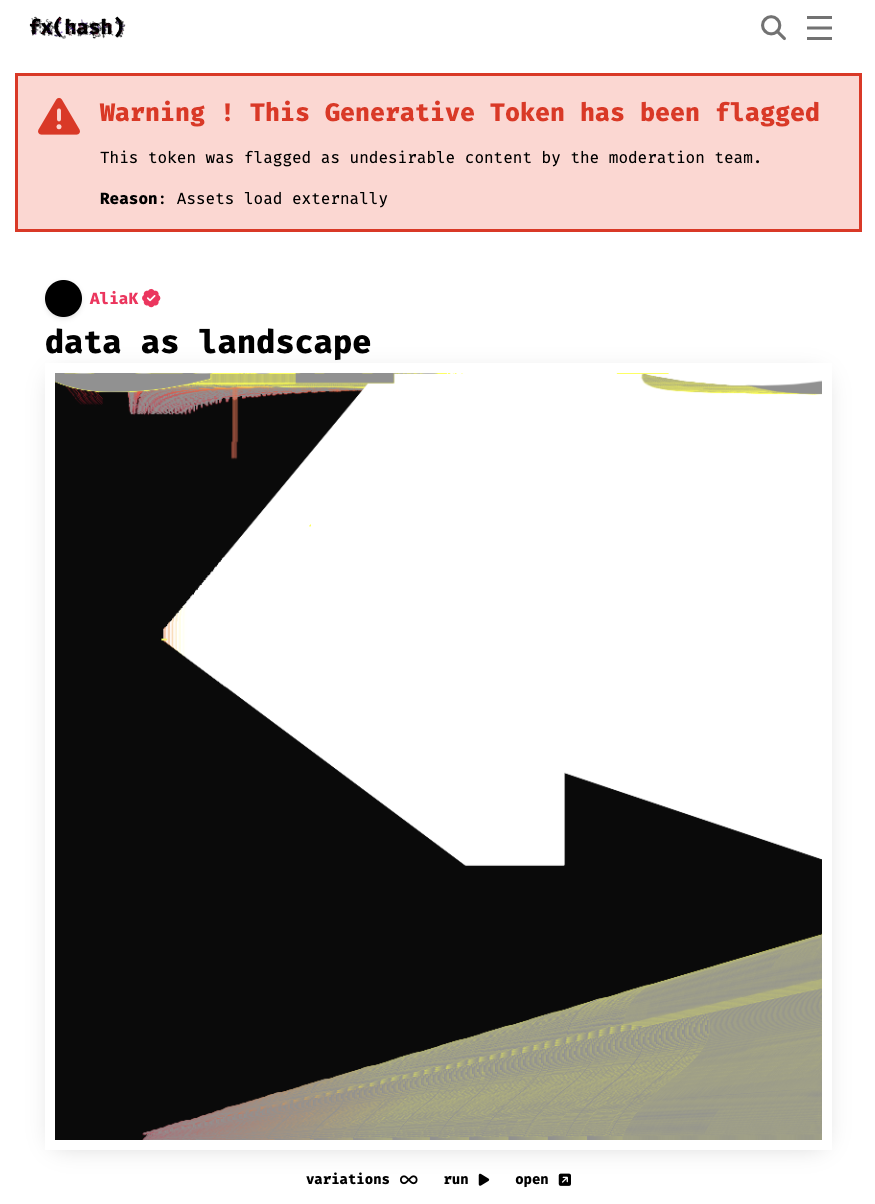
\includegraphics[width=0.5\linewidth]{aliak-data-as-landscape.png}
    \caption[Data as Landscape by AliaK]{Data as Landscape by AliaK, 2022. Source: https://www.fxhash.xyz/generative/13124}
    \label{fig:aliak-data-as-landscape}
\end{figure}



\subsection{Burn it: NFTs as reedemable vouchers}

One of the most common interactions between collectors and projects is the act of collecting and burning tokens as a way to unlock other features in the project, access special drops, or others. Collectors have to weigh in the cost-opportunity of destroying a token in exchange for another which may, or may not, be more desirable for them, both from an economic and aesthetical point of view. Whilst creating an environment of engagement and gamification of the project, it can certainly be considered one of the most striking examples of commodification or art in the NFT world. The very act of permanently disposing of a piece of art in return for some kind of utility is arguably against the very ethos of ``art'' (that which has no utility).

The topic of utility has itself generated a fair amount of debate among the crypto art enthusiasts. TODO: expand on this.



As Innocenti stated, "if conservation for digital art is a moving target, then our scientific methodology should be a moving gun" \citeyear[p.230]{innocentiKeepingBitsAlive2013}.



\section{Theoretical Framework}

\todo rhizome theory

tragedy of the commons \cite{feenyTragedyCommonsTwentytwo1990}

governance \cite{gaziCodeWeTrust2024}


\todo web3 lens: sustainability, or ecosystem ecology






